\documentclass[10pt]{beamer}

\usetheme{metropolis}
\usepackage{booktabs}
\usepackage{amsmath}
\usepackage{graphicx}
\usepackage{tikz}

% Python-inspired color scheme
\definecolor{pythonblue}{RGB}{55,118,171}      % Python blue
\definecolor{pythonyellow}{RGB}{255,212,59}    % Python yellow
\definecolor{pythondarkblue}{RGB}{35,75,110}   % Darker blue for contrast
\definecolor{pythonlightblue}{RGB}{106,159,181} % Lighter blue

% Apply colors to Metropolis theme
\setbeamercolor{frametitle}{bg=pythonblue, fg=white}
\setbeamercolor{progress bar}{fg=pythonyellow, bg=pythonlightblue}
\setbeamercolor{title separator}{fg=pythonyellow}
\setbeamercolor{progress bar in head/foot}{fg=pythonyellow, bg=pythonlightblue}
\setbeamercolor{progress bar in section page}{fg=pythonyellow, bg=pythonlightblue}

% Title page colors
\setbeamercolor{title}{fg=pythonblue}
\setbeamercolor{subtitle}{fg=pythondarkblue}
\setbeamercolor{author}{fg=black}
\setbeamercolor{date}{fg=pythondarkblue}

% Block colors
\setbeamercolor{block title}{bg=pythonblue, fg=white}
\setbeamercolor{block body}{bg=pythonlightblue!20, fg=black}

% Alert and example blocks
\setbeamercolor{block title alerted}{bg=pythonyellow, fg=black}
\setbeamercolor{block body alerted}{bg=pythonyellow!20, fg=black}

% Itemize/enumerate colors
\setbeamercolor{itemize item}{fg=pythonblue}
\setbeamercolor{itemize subitem}{fg=pythonblue}
\setbeamercolor{enumerate item}{fg=pythonblue}

% Standout frames (for section dividers)
\setbeamercolor{standout}{bg=pythonblue, fg=white}

\title{Why Everyone is Talking About GPUs}
\subtitle{The Matrix Multiplication Story}
\date{October 11, 2025}
\author{Your Name}
\institute{MumPy Meetup}

\begin{document}

\maketitle

% Slide 1: NVIDIA Stock - Conversation Starter
\begin{frame}[plain]
  \begin{center}
    \vspace{1em}
    % PLACEHOLDER: Image of NVIDIA stock price chart showing dramatic rise
    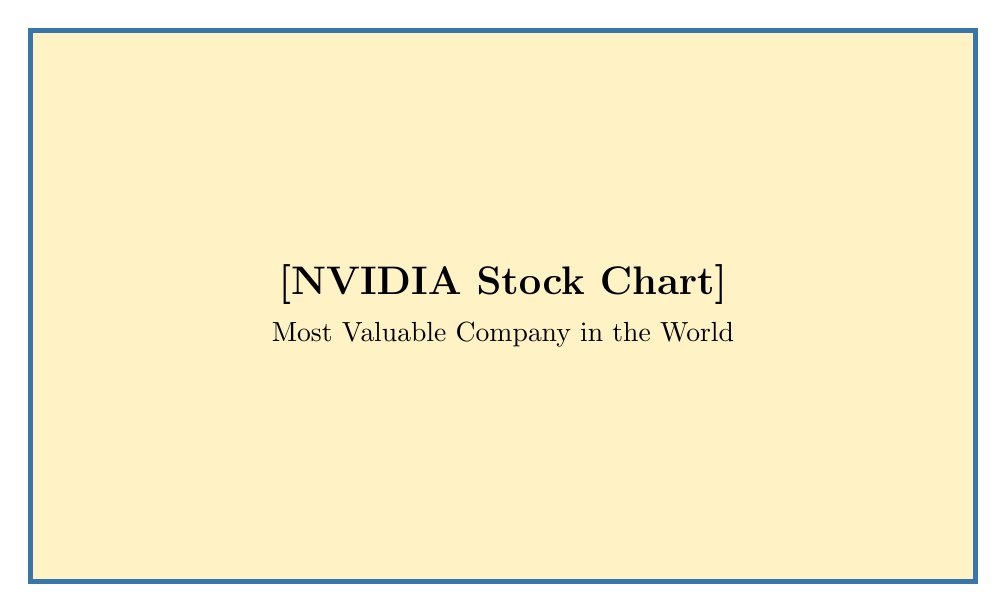
\begin{tikzpicture}
      \draw[fill=pythonyellow!30, draw=pythonblue, line width=2pt] (0,0) rectangle (12,7);
      \node[align=center] at (6,3.5) {\Large\textbf{[NVIDIA Stock Chart]}\\[0.5em]\normalsize Most Valuable Company in the World};
    \end{tikzpicture}
  \end{center}
\end{frame}

% Slide 2: Opening Question
\begin{frame}{GPUs are Everywhere Now}
  \begin{itemize}
    \item ChatGPT needs thousands of GPUs
    \item Image generators like DALL-E run on GPUs
    \item Self-driving cars use GPUs
    \item Gaming has always used GPUs
  \end{itemize}
  
  \vspace{1em}
  \Large \textbf{But why?}
\end{frame}

% Slide 2: A Relatable Problem
\begin{frame}{A Relatable Problem}
  \textbf{Question:} How long will it take me to reach Andheri?
  
  \vspace{1em}
  \begin{center}
    % PLACEHOLDER: Image of Mumbai map with location markers
    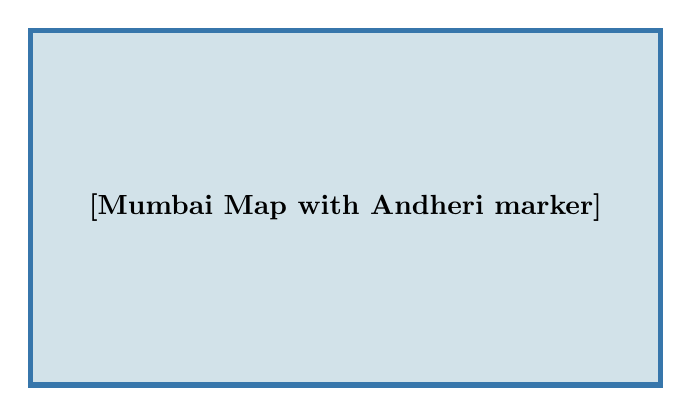
\begin{tikzpicture}
      \draw[fill=pythonlightblue!30, draw=pythonblue, line width=2pt] (0,0) rectangle (8,4.5);
      \node at (4,2.25) {\textbf{[Mumbai Map with Andheri marker]}};
    \end{tikzpicture}
  \end{center}
\end{frame}

% Slide 3: Features We Consider
\begin{frame}{What Affects Travel Time?}
  \begin{columns}[T]
    \begin{column}{0.5\textwidth}
      \begin{itemize}
        \item Distance
        \item Time of day
        \item Is it raining?
        \item Weekday/Weekend
        \item Traffic conditions
        \item Construction zones
      \end{itemize}
    \end{column}
    \begin{column}{0.5\textwidth}
      % PLACEHOLDER: Icons or visual showing these features
      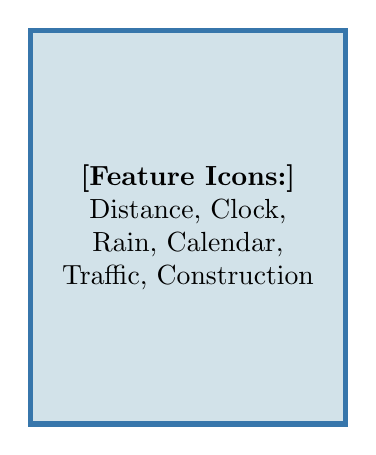
\begin{tikzpicture}
        \draw[fill=pythonlightblue!30, draw=pythonblue, line width=2pt] (0,0) rectangle (4,5);
        \node[align=center] at (2,2.5) {\textbf{[Feature Icons:]}\\Distance, Clock,\\Rain, Calendar,\\Traffic, Construction};
      \end{tikzpicture}
    \end{column}
  \end{columns}
\end{frame}

% Slide 4: Traditional vs ML Approach
\begin{frame}{Two Approaches}
  \begin{block}{Traditional: Rule-Based}
    IF (distance > 10km AND is\_raining) THEN add 30 minutes...
  \end{block}
  
  \vspace{1em}
  
  \begin{block}{Machine Learning}
    Convert everything to numbers, learn a function
  \end{block}
  
  \vspace{1em}
  \small We won't cover the learning part today, just the prediction part!
\end{frame}

% Slide 5: Simple Prediction Formula
\begin{frame}{Making a Prediction}
  For one location, we do:
  
  \vspace{1em}
  \begin{align*}
    \text{predicted\_time} = &\; \text{distance} \times w_1 \\
    &+ \text{time\_of\_day} \times w_2 \\
    &+ \text{is\_raining} \times w_3 \\
    &+ \text{is\_weekend} \times w_4
  \end{align*}
  
  \vspace{1em}
  \small The weights ($w_1, w_2, w_3, w_4$) are learned from data
\end{frame}

% Slide 6: Scaling Up
\begin{frame}{But What If...}
  \begin{itemize}
    \item We have \textbf{50 features} instead of 4?
    \item We want to predict for \textbf{1,000 locations} at once?
    \item We have \textbf{multiple layers} of transformations? (deep learning)
  \end{itemize}
  
  \vspace{2em}
  \centering
  \Large This becomes \textbf{matrix multiplication}
\end{frame}

% Slide 7: Matrix Multiplication
\begin{frame}{Matrix Multiplication}
  \begin{center}
    % PLACEHOLDER: Visual showing matrix multiplication with dimensions labeled
    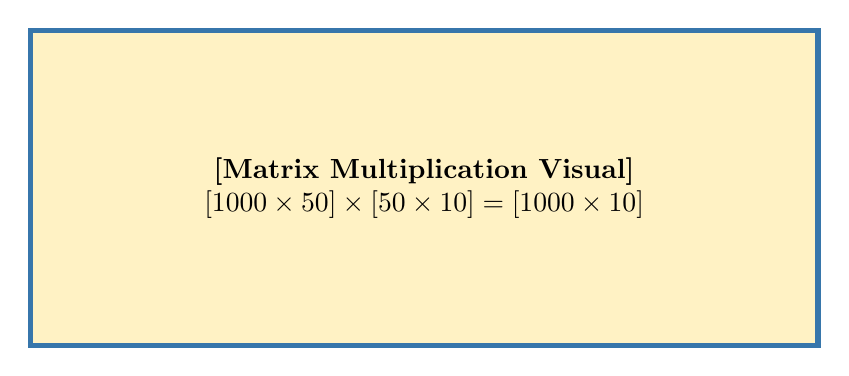
\begin{tikzpicture}
      \draw[fill=pythonyellow!30, draw=pythonblue, line width=2pt] (0,0) rectangle (10,4);
      \node[align=center] at (5,2) {\textbf{[Matrix Multiplication Visual]}\\$[1000 \times 50] \times [50 \times 10] = [1000 \times 10]$};
    \end{tikzpicture}
  \end{center}
  
  \vspace{0.5em}
  \centering
  \small Interactive demo: \texttt{http://matrixmultiplication.xyz/}
\end{frame}

% Slide 8: The Scale
\begin{frame}{The Real Scale}
  \textbf{Modern ML models:}
  
  \vspace{1em}
  \begin{itemize}
    \item GPT-3: 175 \textbf{billion} parameters
    \item Billions of multiply-add operations per prediction
    \item Training involves trillions of operations
  \end{itemize}
  
  \vspace{2em}
  \centering
  \Large How do we compute this efficiently?
\end{frame}

% Slide 9: CPU Architecture
\begin{frame}{CPU: The Generalist}
  \begin{columns}[T]
    \begin{column}{0.5\textwidth}
      \textbf{Few powerful cores}
      \begin{itemize}
        \item 4-16 cores typically
        \item Sequential processing
        \item Great for general tasks
      \end{itemize}
      
      \vspace{1em}
      \textbf{Analogy:} 8 very smart people solving 10,000 problems one by one
    \end{column}
    \begin{column}{0.5\textwidth}
      % PLACEHOLDER: Diagram of CPU architecture
      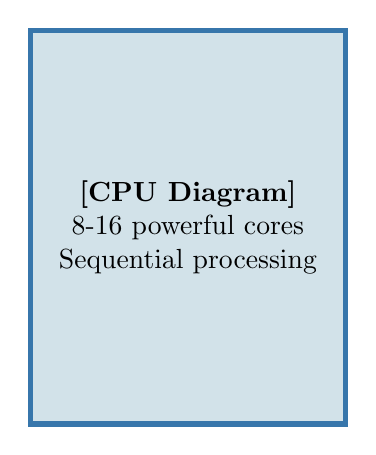
\begin{tikzpicture}
        \draw[fill=pythonlightblue!30, draw=pythonblue, line width=2pt] (0,0) rectangle (4,5);
        \node[align=center] at (2,2.5) {\textbf{[CPU Diagram]}\\8-16 powerful cores\\Sequential processing};
      \end{tikzpicture}
    \end{column}
  \end{columns}
\end{frame}

% Slide 10: CPU Limitation
\begin{frame}{The CPU Bottleneck}
  \begin{center}
    % PLACEHOLDER: Animation/diagram showing CPU doing matrix mult sequentially
    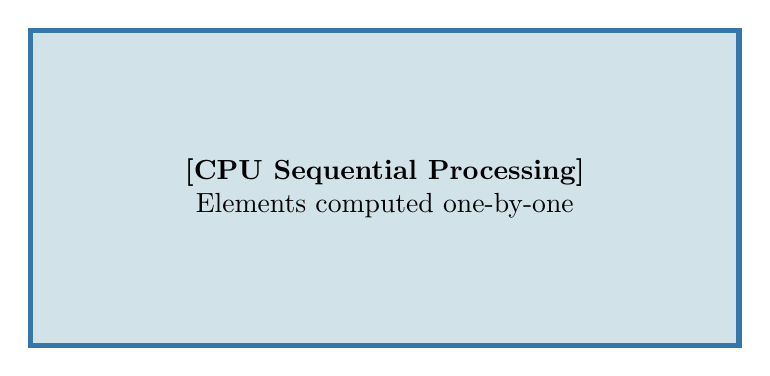
\begin{tikzpicture}
      \draw[fill=pythonlightblue!30, draw=pythonblue, line width=2pt] (0,0) rectangle (9,4);
      \node[align=center] at (4.5,2) {\textbf{[CPU Sequential Processing]}\\Elements computed one-by-one};
    \end{tikzpicture}
  \end{center}
  
  \vspace{1em}
  \centering
  Matrix multiplication is \textbf{inherently parallel}, but CPU does it \textbf{sequentially}
\end{frame}

% Slide 11: GPU Architecture
\begin{frame}{GPU: The Parallel Powerhouse}
  \begin{columns}[T]
    \begin{column}{0.5\textwidth}
      \textbf{Thousands of smaller cores}
      \begin{itemize}
        \item 10,000+ CUDA cores
        \item Parallel processing
        \item Specialized for repetitive tasks
      \end{itemize}
      
      \vspace{1em}
      \textbf{Analogy:} 10,000 people each solving one problem simultaneously
    \end{column}
    \begin{column}{0.5\textwidth}
      % PLACEHOLDER: Diagram of GPU architecture
      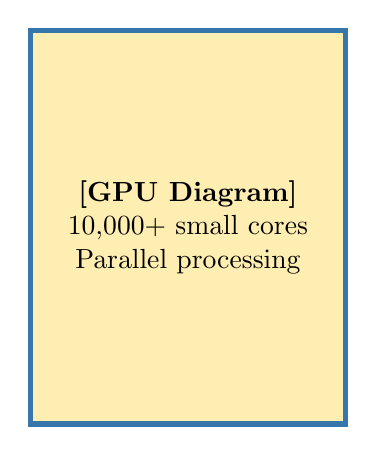
\begin{tikzpicture}
        \draw[fill=pythonyellow!40, draw=pythonblue, line width=2pt] (0,0) rectangle (4,5);
        \node[align=center] at (2,2.5) {\textbf{[GPU Diagram]}\\10,000+ small cores\\Parallel processing};
      \end{tikzpicture}
    \end{column}
  \end{columns}
\end{frame}

% Slide 12: GPU Parallel Processing
\begin{frame}{Parallel Matrix Multiplication}
  \begin{center}
    % PLACEHOLDER: Animation/diagram showing GPU doing matrix mult in parallel
    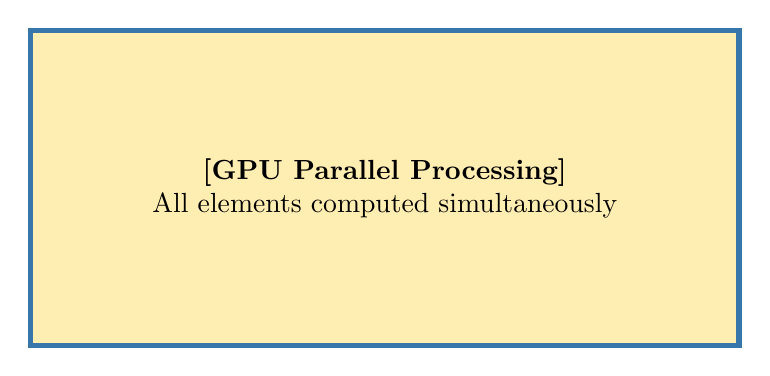
\begin{tikzpicture}
      \draw[fill=pythonyellow!40, draw=pythonblue, line width=2pt] (0,0) rectangle (9,4);
      \node[align=center] at (4.5,2) {\textbf{[GPU Parallel Processing]}\\All elements computed simultaneously};
    \end{tikzpicture}
  \end{center}
  
  \vspace{1em}
  \centering
  Each element computed \textbf{simultaneously}!
\end{frame}

% Slide 13: Why GPUs Originally
\begin{frame}{Why GPUs Exist}
  GPUs were originally designed for \textbf{graphics and gaming}
  
  \vspace{1em}
  \begin{itemize}
    \item 3D transformations: matrix operations
    \item Rendering millions of pixels: parallel
    \item Real-time requirements: fast
  \end{itemize}
  
  \vspace{1em}
  \centering
  \textbf{Turns out:} AI has the same needs!
\end{frame}

% Slide 14: Demo Section Title
\begin{frame}[standout]
  \Huge Seeing is Believing
  
  \vspace{1em}
  \Large Python Timing Examples
\end{frame}

% Slide 15: Demo 1 Setup
\begin{frame}[fragile]{Demo 1: NumPy vs CuPy}
  \textbf{Setup:} Large matrix multiplication
  
  \vspace{0.5em}
  \begin{columns}[T]
    \begin{column}{0.48\textwidth}
      \textbf{CPU (NumPy)}
      \tiny
\begin{verbatim}
import numpy as np
import time

size = 10000
A = np.random.rand(size, size)
B = np.random.rand(size, size)

start = time.time()
C = A @ B
end = time.time()

print(f"Time: {end-start:.2f}s")
\end{verbatim}
    \end{column}
    \begin{column}{0.48\textwidth}
      \textbf{GPU (CuPy)}
      \tiny
\begin{verbatim}
import cupy as cp
import time

size = 10000
A = cp.random.rand(size, size)
B = cp.random.rand(size, size)

start = time.time()
C = A @ B
cp.cuda.Stream.null.synchronize()
end = time.time()

print(f"Time: {end-start:.2f}s")
\end{verbatim}
    \end{column}
  \end{columns}
\end{frame}

% Slide 16: Demo 1 Results
\begin{frame}{Demo 1: Results}
  \begin{center}
    % PLACEHOLDER: Bar chart comparing NumPy vs CuPy timing
    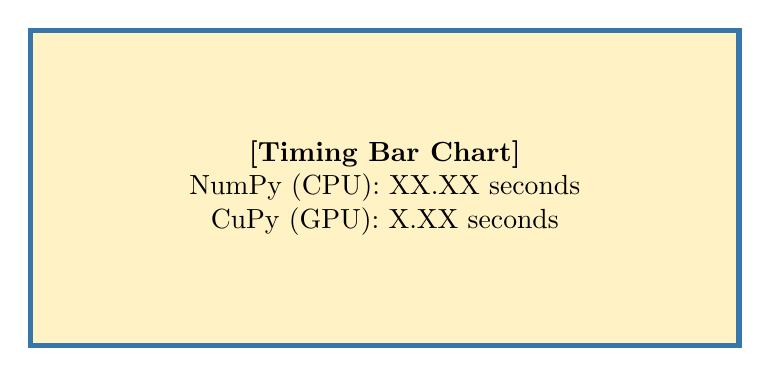
\begin{tikzpicture}
      \draw[fill=pythonyellow!30, draw=pythonblue, line width=2pt] (0,0) rectangle (9,4);
      \node[align=center] at (4.5,2) {\textbf{[Timing Bar Chart]}\\NumPy (CPU): XX.XX seconds\\CuPy (GPU): X.XX seconds};
    \end{tikzpicture}
  \end{center}
  
  \vspace{1em}
  \centering
  \Large \textbf{50-100x speedup} on GPU!
\end{frame}

% Slide 17: Demo 2 Setup
\begin{frame}[fragile]{Demo 2: PyTorch CPU vs GPU}
  \textbf{Setup:} Neural network forward pass
  
  \vspace{0.5em}
  \tiny
\begin{verbatim}
import torch
import torch.nn as nn

# Create a simple neural network
model = nn.Sequential(
    nn.Linear(1000, 5000),
    nn.ReLU(),
    nn.Linear(5000, 5000),
    nn.ReLU(),
    nn.Linear(5000, 1000)
)

# Input data
x = torch.randn(1000, 1000)

# CPU version                          # GPU version
model_cpu = model.to('cpu')            model_gpu = model.to('cuda')
x_cpu = x.to('cpu')                    x_gpu = x.to('cuda')
output = model_cpu(x_cpu)              output = model_gpu(x_gpu)
\end{verbatim}
\end{frame}

% Slide 18: Demo 2 Results
\begin{frame}{Demo 2: Results}
  \begin{center}
    % PLACEHOLDER: Bar chart comparing PyTorch CPU vs GPU timing
    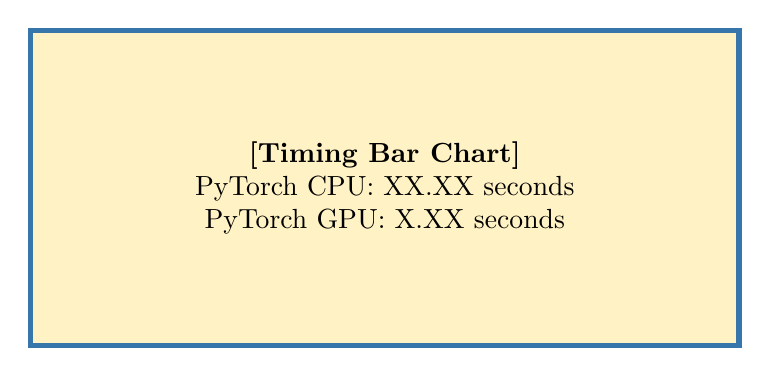
\begin{tikzpicture}
      \draw[fill=pythonyellow!30, draw=pythonblue, line width=2pt] (0,0) rectangle (9,4);
      \node[align=center] at (4.5,2) {\textbf{[Timing Bar Chart]}\\PyTorch CPU: XX.XX seconds\\PyTorch GPU: X.XX seconds};
    \end{tikzpicture}
  \end{center}
  
  \vspace{1em}
  \centering
  \Large \textbf{100-200x speedup} for deep learning!
\end{frame}

% Slide 19: When Should You Care?
\begin{frame}{When Should You Care About GPUs?}
  \textbf{Use GPUs when you have:}
  
  \vspace{1em}
  \begin{itemize}
    \item Large matrices (thousands of rows/columns)
    \item Repeated operations (training loops)
    \item Real-time requirements
    \item Deep learning models
  \end{itemize}
  
  \vspace{1em}
  \textbf{Skip GPUs for:}
  \begin{itemize}
    \item Small data (< 1000 elements)
    \item One-off calculations
    \item Overhead of data transfer > computation time
  \end{itemize}
\end{frame}

% Slide 20: How to Get Started
\begin{frame}{How to Get Started}
  \textbf{Free options:}
  \begin{itemize}
    \item \textbf{Google Colab} - Free T4 GPU access
    \item \textbf{Kaggle Notebooks} - Free GPU hours
  \end{itemize}
  
  \vspace{1em}
  \textbf{Cloud providers:}
  \begin{itemize}
    \item AWS, Google Cloud, Azure
    \item Pay per hour of GPU usage
  \end{itemize}
  
  \vspace{1em}
  \textbf{Local GPU:}
  \begin{itemize}
    \item NVIDIA GPUs (required for CUDA)
    \item For serious/regular ML work
  \end{itemize}
\end{frame}

% Slide 21: Python Tools
\begin{frame}{Python Tools for GPU Computing}
  \begin{description}
    \item[PyTorch] Most popular for deep learning, easy GPU support
    \item[TensorFlow] Google's framework, mature ecosystem
    \item[CuPy] NumPy, but on GPU
    \item[JAX] Google's new framework, automatic differentiation
    \item[RAPIDS] GPU-accelerated data science (pandas-like)
  \end{description}
  
  \vspace{1em}
  \centering
  \small Most just need \texttt{.to('cuda')} or similar!
\end{frame}

% Slide 22: Summary
\begin{frame}{Putting It All Together}
  \begin{enumerate}
    \item Modern AI = \textbf{lots of matrix multiplication}
    \item Matrix multiplication = \textbf{embarrassingly parallel}
    \item CPUs = sequential, GPUs = \textbf{parallel powerhouses}
    \item Result: \textbf{50-200x speedup} for ML workloads
  \end{enumerate}
  
  \vspace{2em}
  \centering
  \Large That's why every AI breakthrough mentions "GPU hours"!
\end{frame}

% Slide 23: Thank You
\begin{frame}[standout]
  \Huge Thank You!
  
  \vspace{2em}
  \Large Questions?
  
  \vspace{2em}
  \normalsize
  Demo: \texttt{http://matrixmultiplication.xyz/}
\end{frame}

\end{document}

